% ====================================================================
% MAT-305 PWA 1 Report
% Jake Killian | XeLaTeX build
% ====================================================================

% --------------------------------------------------------------------
% Core document configuration
% --------------------------------------------------------------------
\documentclass[12pt]{article} % Requires XeLaTeX or LuaLaTeX for fontspec

% --------------------------------------------------------------------
% Font and math configuration (system font stack + Unicode math)
% --------------------------------------------------------------------
\usepackage{fontspec}                      % System font access
\usepackage{amsmath}
\usepackage{mathtools}
\usepackage{unicode-math}                  % Unicode-aware math layer

\setmainfont{Libertinus Serif}             % Body text
\setsansfont{Libertinus Sans}              % Sans-serif accents
\setmonofont{JetBrains Mono}[
    Contextuals=Alternate,
    Ligatures=TeX,
    Scale=MatchLowercase
]                                            % Monospaced/code font
\setmathfont{Libertinus Math}              % Math companion to Libertinus

% --------------------------------------------------------------------
% Page geometry, titling, and headers/footers
% --------------------------------------------------------------------
\usepackage[margin=1in]{geometry}
\usepackage{titling}                       % Allows custom title block spacing
\usepackage{fancyhdr}                      % Header/footer branding
\setlength{\headheight}{15.5pt}           % Match colored header rule height
\pagestyle{fancy}
\fancyhf{}

% --------------------------------------------------------------------
% Micro-typography and color palette
% --------------------------------------------------------------------
\usepackage[protrusion=true]{microtype}    % Character protrusion (safe for XeLaTeX)
\usepackage[dvipsnames]{xcolor}            % Extended color names for palette

\definecolor{AccentColor}{HTML}{7B1113}    % Deep Oxide Red
\definecolor{AccentMuted}{HTML}{5C0D0F}    % Darker variant
\definecolor{AccentInk}{HTML}{111111}      % Charcoal gray (reserved for text if needed)
\definecolor{Highlighter}{HTML}{FFF59D}    % Soft yellow highlight
\definecolor{Alert}{HTML}{D32F2F}          % Strong alert red

% --------------------------------------------------------------------
% Math helpers and scientific formatting
% --------------------------------------------------------------------
\usepackage{cancel}                        % Strike through terms in derivations
\renewcommand{\CancelColor}{\color{red}}

\usepackage{siunitx}                       % Consistent scientific units
\sisetup{
    detect-all,
    per-mode = symbol,
    separate-uncertainty = true,
    exponent-product = \cdot
}

% --------------------------------------------------------------------
% Figures, plotting, and tables
% --------------------------------------------------------------------
\usepackage{graphicx}
\usepackage{float}
\usepackage{caption}                       % Required before subcaption
\usepackage{subcaption}
\usepackage{pgfplots}
\pgfplotsset{compat=1.18}
\usepackage{pgfplotstable}

\usepackage{booktabs}
\usepackage{array}
\usepackage{tabularx}
\usepackage{multirow}
\usepackage{makecell}
\usepackage{csvsimple}

% --------------------------------------------------------------------
% Lists, hyperlinks, and references
% --------------------------------------------------------------------
\usepackage{enumitem}
\usepackage[hidelinks]{hyperref}
\usepackage[nameinlink,capitalise,noabbrev]{cleveref}

% --------------------------------------------------------------------
% Attachments and PDF utilities
% --------------------------------------------------------------------
\usepackage{pdfpages}
\usepackage{attachfile2}                   % Embed supplemental files inside PDF

% --------------------------------------------------------------------
% Spacing, paragraph handling, and quotations
% --------------------------------------------------------------------
\usepackage{setspace}
\singlespacing
\usepackage{indentfirst}                   % Indent first paragraph of each section
\setlength{\parindent}{1.5em}
\usepackage[autostyle,english=american]{csquotes}
\usepackage{listings}

% --------------------------------------------------------------------
% Default stylistic settings
% --------------------------------------------------------------------
\numberwithin{equation}{section}
\captionsetup{labelfont=bf}
\setlist{itemsep=0.25em, topsep=0.25em}

% --------------------------------------------------------------------
% Personalization toggle (enables branded header when true)
% --------------------------------------------------------------------
\newif\ifpersonal
\personaltrue

\ifpersonal
    \lhead{\textcolor{AccentColor!80!black}{Jake Killian}}
    \rhead{\textcolor{gray}{\leftmark}}
    \cfoot{\textcolor{gray}{\thepage}}
\else
    \rhead{\leftmark}
    \cfoot{\thepage}
\fi

% --------------------------------------------------------------------
% Section heading styling (underline motif below each heading)
% --------------------------------------------------------------------
\usepackage[explicit]{titlesec}

\newcommand{\sectionline}{%                % Underline accent for \section
    \par\vspace{0.1em}\noindent{\color{AccentMuted}\rule{2cm}{0.6pt}}\par
}
\newcommand{\subsectionline}{%             % Underline accent for \subsection
    \par\vspace{0.1em}\noindent{\color{AccentMuted}\rule{1.5cm}{0.5pt}}\par
}

\ifpersonal
    \titleformat{\section}
        {\LARGE\bfseries\color{AccentColor}}
        {\thesection}{0.75em}{#1\sectionline}
    \titlespacing*{\section}{0pt}{1.5ex plus 0.5ex minus 0.2ex}{1.0ex}

    \titleformat{\subsection}
        {\large\bfseries\color{AccentColor!85!black}}
        {\thesubsection}{0.6em}{#1\subsectionline}
    \titlespacing*{\subsection}{0pt}{1.0ex plus 0.4ex minus 0.2ex}{0.8ex}
\else
    \titleformat{\section}
        {\Large\bfseries}
        {\thesection}{0.75em}{#1\sectionline}
    \titleformat{\subsection}
        {\large\bfseries}
        {\thesubsection}{0.6em}{#1\subsectionline}
\fi

% --------------------------------------------------------------------
% Inline emphasis helpers
% --------------------------------------------------------------------
\newcommand{\highlight}[1]{\colorbox{Highlighter}{#1}}
\newcommand{\important}[1]{\textcolor{Alert}{\textbf{#1}}}

% --------------------------------------------------------------------
% Hyperref colorization
% --------------------------------------------------------------------
\hypersetup{
    colorlinks=true,
    linkcolor=AccentMuted,
    citecolor=AccentMuted,
    urlcolor=AccentColor
}

% --------------------------------------------------------------------
% Title block helper (colored rule beneath \maketitle)
% --------------------------------------------------------------------
\providecommand{\PrintTitleRule}{}
\renewcommand{\PrintTitleRule}{%
    \par\medskip
    \begin{center}
        {\color{AccentColor}\rule{0.6\linewidth}{0.6pt}}%
    \end{center}
    \par\medskip
}

% --------------------------------------------------------------------
% Fancyhdr tuning (colored rule + section marks)
% --------------------------------------------------------------------
\renewcommand{\sectionmark}[1]{\markboth{#1}{}}

\makeatletter
\renewcommand{\headrulewidth}{0.6pt}
\def\headrule{% Draw the colored rule once per header
    {\color{AccentMuted}\hrule\@height\headrulewidth\@width\headwidth\relax}%
}
\makeatother

% --------------------------------------------------------------------
% Title metadata
% --------------------------------------------------------------------
\pretitle{\begin{center}\LARGE}
\title{MAT-305 - PWA 1}
\posttitle{\par\smallskip\Large Chapter 9: \textit{Persistence}\par\end{center}}
\preauthor{\begin{center}\large}
\author{Jake Killian}
\postauthor{\par\end{center}}
\predate{\begin{center}\large}
\date{October 10, 2025}
\postdate{\par\end{center}}

\begin{document}

\maketitle
\PrintTitleRule

\section{Personal Experiences with Failure}
    \begin{enumerate}[label = (\alph*)]
        \item What was something outside of coursework that you tried and failed at?
            What was the experience like?
            Were you hard on yourself?
            Were you understanding that you won't succeed at everything immediately?
            What, if anything, did you learn from it?\par
            \smallskip
            \hspace{0.5em}
            \textbf{Response:}\par
            \indent Something outside of coursework that I have so far tried and failed at is properly leaning to accept failure.
            I have always been a perfectionist and have a hard time accepting failure in any capacity.
            When I fail at something, I tend to either completely not care and move on or repeat the task over and over until I succeed.
            I understand that binarily choosing to either care too much or not at all is not a healthy way to approach failure.
            I am still working on finding a middle ground where I can accept failure as a natural part of life.
            My inability to accept failure has caused me to miss out on opportunities because I was too afraid of the possibility of failing.
            Examples of this range from me largely avoiding playing competitive games because I view losing as failure to not talking to people I find interesting because I view rejection as failure.
            I am overtly hard on myself when I fail at something.
            I understand that I may not be able to succeed at everything immediately, but I still get frustrated when I don't succeed initially.
            It bothers me enough that I will often repeat the task until success, even if it is detrimental to myself to do so.
            I am still learning to accept failure as a natural part of life.
            I am trying to view failure more so as a learning opportunity rather than a negative experience.
\pagebreak[3]
        \item What was something related to coursework that you tried and failed at?
            This could be misunderstanding a concept or a procedure.
            It could be trying out an alternative method that turned out to not work.
            \textit{Don't tell me that you made an algebra error; that is more of a small "slip" and not "failure".}
            What was the experience like and how did you respond?
            Was your response to an academic failure different than a non-academic one?
            What, if anything, did you learn from it?\par
            \smallskip
            \hspace{0.5em}
            \textbf{Response:}\par
            \indent Something related to coursework that I have tried and failed at is learning how to properly manage my time.
            I have always struggled with procrastination, overcommitting myself, and poor planning.
            Although I like to think I produce high quality work, I often find that this can come at the cost of time.
            My perfectionism often leads me to spend too much time on assignments, which can result in me rushing to complete other tasks or not completing them at all.
            To elaborate on that last point, I have a tendency to either submit my assignments on time or not at all, because I would rather not submit something than submit something that I am not proud of.
            This issue has caused me to miss deadlines and has impacted my academic performance.
            I am still actively working on improving my time management skills.
            I attempt to do this by trying new time management strategies when the current strategy I am using is not working well.
            My response to this failure is similar to my response to non-academic failures, in that I tend to either not care or care too much.
            This binary behavior is consistent with my general response to failure, and is something that I am actively trying to improve.
            I am learning that I may not be able to do everything perfectly given external constraints, and that is okay.
            I am also learning to find a balance between caring too much and not at all.
\pagebreak[3]
        \item Failure in mathematics often makes people feel "stupid" whereas failure in other disciplines (e.g., history, languages, art, etc.) or failures in everyday life do not always seem to carry the same weight.
            Of course, math is just like anything else, it requires practice and patience to be good at, and everyone who does mathematics has experienced failures, so why do you think that message persists?
            Who does it benefit and who might it harm?
            What are some ways that you can resist equating mathematical failure with lack of intelligence, and instead view it as a necessary part of the process of coming to understand new things?
            (For instance, what's something you might try the next time you experience failure?)\par
            \smallskip
            \hspace{0.5em}
            \textbf{Response:}\par
            \indent I think the message/idea that failure in mathematics is somehow correlated with a lack of intelligence persists because of both the societal stereotype that mathematical ability is correlated to intelligence and the fact that mathematics is often viewed as having a binary right or wrong answer.
            I think the stereotype around math and intelligence exists because of the historical emphasis on mathematics as a measure of intelligence.
            This stereotype is perpetuated by our education system and by society as a whole.
            Being wrong in math is often harder to accept because of the binary nature of math.
            Although there are often multiple ways to solve a problem, there is typically only one correct answer.
            Being wrong in math usually indicates a failure in process or understanding, and should not be thought of as a lack of intelligence.
            I think this stereotype benefits those who are already good at math, as it increases their perceived intelligence and status among peers.
            I think this stereotype harms both those who struggle at math and those who are good at math.
            The stereotype creates unnecessary pressure and anxiety for those who struggle, but also those who are good at math as they may feel that they have to maintain a minimum level of proficiency, otherwise they could be considered a failure.
            A perceived lack of intelligence can also lead to reduced confidence and self-esteem.
            Some ways we can resist equating mathematical failure with lack of intelligence is by recognizing that failure is a natural part of the learning process and that everyone experiences it.
            We should also not only look at the final answer and the binary nature of its correctness, but also at the process which led to that answer.
            Failure is an opportunity to learn and grow, and should be viewed as such.
            Next time I experience failure, I will try to take a step back and analyze what went wrong in the process, rather than focusing only on the incorrect result.
            Failure means something can be improved or fixed, not that the entire person, their intelligence, or the attempt is a failure.
            We should ask ourselves how we can better ourselves instead of classifying ourselves as failures.
\pagebreak[3]
    \end{enumerate}

\pagebreak[4]
\section{Problem Analysis \& Solutions}
    \indent A collection of solar panels is mounted on the roof of a house.
    The panel may be regarded as positioned at the points of coordinates (in meters) \(A(4, 0, 0)\), \(B(4, 11, 0)\), \(C(0, 11, 4)\), and \(D(0, 0, 4)\).
    See Figure~\ref{fig:solar-panels} below.
    \medskip
    \begin{figure}[H]
        \centering
        \IfFileExists{../figures/PWA-1_solar-panels.png}{%
            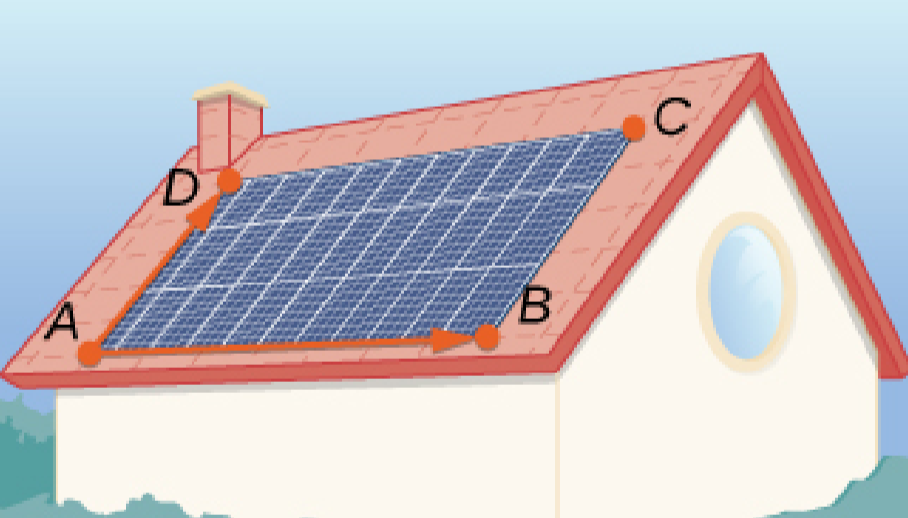
\includegraphics[width=0.5\linewidth]{../figures/PWA-1_solar-panels.png}%
        }{%
            \fbox{\parbox{0.5\linewidth}{\centering Missing figure: PWA-1\_solar-panels.png}}%
        }
        \caption{Solar panel placement on the roof of a house}
        \label{fig:solar-panels}
    \end{figure}
\pagebreak[3]
    \begin{enumerate}[label=\roman*.]
    \item Find a vector \(n\) perpendicular to the surface of solar panels.
            Then use it to compute the area taken up by the solar panels on the roof of the house.\par
            \bigskip
            \hspace{0.5em}
            \textbf{Analysis \& Solution:}
            \begin{center}
            \rule{\linewidth}{1pt}
            \end{center}
            \begin{enumerate}[label=\arabic*.]
                \item First we need to establish the locations of the corners of the solar panel array.
                    From our problem statement, we are given the coordinates of the corners as:
                    \[
                    A = (4, 0, 0), \quad B = (4, 11, 0), \quad C = (0, 11, 4), \quad D = (0, 0, 4).
                    \]
                \item We next need to find two vectors that lie on the plane of the solar panel array.
                    In this case, we can use the vectors \(\overrightarrow{AB}\) and \(\overrightarrow{AD}\).
                    These vectors are displacement vectors from point \(A\) to points \(B\) and \(D\) respectively.
                    To find these displacement vectors, we subtract the coordinates of point \(A\) from the coordinates of points \(B\) and \(D\):
                    \[
                    \overrightarrow{AB} = B - A = (4 - 4, 11 - 0, 0 - 0)
                    \]
                    \[
                    \overrightarrow{AB} = (0, 11, 0)
                    \]
                    \smallskip
                    \[
                    \overrightarrow{AD} = D - A = (0 - 4, 0 - 0, 4 - 0)
                    \]
                    \[
                    \overrightarrow{AD} = (-4, 0, 4)
                    \]
                \item Now that we have two vectors on our plane of interest, we can find a normal vector \(\vec{n}\) to the plane by taking the cross product of \(\overrightarrow{AB}\) and \(\overrightarrow{AD}\):
                    \[
                    \vec{n} = \overrightarrow{AB} \times \overrightarrow{AD}
                    \]
                    To compute this cross product, we can use the determinant of the matrix formed by the unit vectors \(\boldsymbol{\hat{\imath}}\), \(\boldsymbol{\hat{\jmath}}\), \(\boldsymbol{\hat{k}}\) and the components of our two vectors:
                    \[
                    \vec{n} = \begin{vmatrix}
                    \boldsymbol{\hat{\imath}} & \boldsymbol{\hat{\jmath}} & \boldsymbol{\hat{k}} \\
                    0 & 11 & 0 \\
                    -4 & 0 & 4
                    \end{vmatrix}
                    \]
                    To solve for this determinant, we expand it as follows:
                    \[
                    \vec{n} = ((11) (4) - (0) (0))\boldsymbol{\hat{\imath}} - ((0) (4) - (-4) (0))\boldsymbol{\hat{\jmath}} + ((0) (0) - (-4) (11))\boldsymbol{\hat{k}}
                    \]
                    Simplifying, we get:
                    \[
                    \vec{n} = (44)\boldsymbol{\hat{\imath}} - (0)\boldsymbol{\hat{\jmath}} + (44)\boldsymbol{\hat{k}} = \left\langle 44, 0, 44 \right\rangle
                    \]
                    We can express our final answer for the normal vector in component form as:
                    \[
                    \boxed{\vec{n} = \left\langle 44, 0, 44 \right\rangle}
                    \]
                \item Recall that the magnitude of the normal vector \(\vec{n}\) gives us the area of the parallelogram formed by the vectors \(\overrightarrow{AB}\) and \(\overrightarrow{AD}\).
                    To find the magnitude, we use the formula:
                    \[
                    \lVert \vec{n} \rVert = \sqrt{n_x^2 + n_y^2 + n_z^2}
                    \]
                    where \(n_x\), \(n_y\), and \(n_z\) are the components of the vector \(\vec{n}\).
                \item We can identify the components of \(\vec{n}\) by recalling the composition of vector component form:
                    \[
                    \left\langle n_x, n_y, n_z \right\rangle
                    \]
                \item Now we can identify the components of \(\vec{n}\) as:
                    \[
                    n_x = 44, \quad n_y = 0, \quad n_z = 44
                    \]
                \item We can now substitute these values into the formula for the magnitude of \(\vec{n}\):
                    \[
                    \lVert \vec{n} \rVert = \sqrt{44^2 + 0^2 + 44^2}
                    \]
                    \[
                    \lVert \vec{n} \rVert = \sqrt{1936 + 0 + 1936}
                    \]
                    \[
                    \lVert \vec{n} \rVert = \sqrt{3872}
                    \]
                    \[
                    \lVert \vec{n} \rVert \approx 62.24
                    \]
                    Applying the proper units, we find that the area of the solar panels is approximately:
                    \[
                    \boxed{\SI{62.24}{\meter^2}}
                    \]
            \end{enumerate}
\pagebreak[3]
            \begin{center}
            \rule{\linewidth}{0.1pt}
            \end{center}
            \hspace{0.5em}
            \textbf{\textit{Solutions:}}
            \begin{itemize}
                \item Normal vector to the plane on which the solar panels lie:
                    \[
                    \boxed{\vec{n} = \left\langle 44, 0, 44 \right\rangle}
                    \]
                \item Solar panel area:
                    \[
                    \boxed{A_{\text{solar panels}}\approx \SI{62.24}{\meter^2}}
                    \]
            \end{itemize}
            \begin{center}
            \rule{\linewidth}{1pt}
            \end{center}
\pagebreak[3]
        \item Find an equation of the plane on which the solar panels lie.
            You may use any form of plane equation that you like.\par
            \bigskip
            \hspace{0.5em}
            \textbf{Analysis \& Solution:}
            \begin{center}
            \rule{\linewidth}{1pt}
            \end{center}
            \begin{enumerate}[label=\arabic*.]
                \item To find an equation of the plane on which the solar panels lie, we first need to select an equation form.
                    In this case, we will select the point-normal form of the plane equation.
                    This form is given by:
                    \[
                    n_x(x - x_0) + n_y(y - y_0) + n_z(z - z_0) = 0
                    \]
                    where \((x_0, y_0, z_0)\) is a point on the plane and \((n_x, n_y, n_z)\) are the components of the normal vector \(\vec{n}\).
                \item In this example we will use point \(A = (4, 0, 0)\) as our point on the plane.
                    Using our normal vector \(\vec{n} = \left\langle 44, 0, 44 \right\rangle\), (which we found in part (i)), we can again identify the vector components as:
                    \[
                    n_x = 44, \quad n_y = 0, \quad n_z = 44
                    \]
                \item Substituting these values into the point-normal form of the plane equation, we can calculate:
                    \[
                    44(x - 4) + 0(y - 0) + 44(z - 0) = 0
                    \]
                    Simplifying this equation, we obtain the following:
                    \[
                    44x + 44z - 176 = 0
                    \]
                    Simplifying further, we can now write the equation of the plane on which the solar panels lie as:
                    \[
                    \boxed{x + z = 4}
                    \]
            \end{enumerate}
\pagebreak[3]
            \begin{center}
            \rule{\linewidth}{0.1pt}
            \end{center}
            \hspace{0.5em}
            \textbf{\textit{Solutions:}}
            \begin{itemize}
                \item Equation of the plane on which the solar panels lie:
                    \[
                    \boxed{x + z = 4}
                    \]
            \end{itemize}
            \begin{center}
            \rule{\linewidth}{1pt}
            \end{center}
\pagebreak[3]
        \item We have seen that \textit{work} is given by the dot product of force and displacement.
            Here, we will see another application of the dot product in computing \textit{power}.
            Suppose the sun is located along the unit vector \(\textbf{s} = \frac{1}{\sqrt{3}}\boldsymbol{\hat{\imath}} + \frac{1}{\sqrt{3}}\boldsymbol{\hat{\jmath}} + \frac{1}{\sqrt{3}}\boldsymbol{\hat{k}}\) and that the flow of solar energy is given by the vector \(\textbf{F} = 900\textbf{s}\), with units of \(Watts/m^2\).
            Compute the dot product \(\textbf{F} \cdot \textbf{n}\).
            This is the amount of electrical power the solar panels can produce!\par
            \bigskip
            \hspace{0.5em}
            \textbf{Analysis \& Solution:}
            \begin{center}
            \rule{\linewidth}{1pt}
            \end{center}
            \begin{enumerate}[label=\arabic*.]
                \item First, we need to compute the vector \(\vec{F}\).
                    Given that \(\vec{F} = 900\vec{s}\) and \(\vec{s} = \frac{1}{\sqrt{3}}\boldsymbol{\hat{\imath}} + \frac{1}{\sqrt{3}}\boldsymbol{\hat{\jmath}} + \frac{1}{\sqrt{3}}\boldsymbol{\hat{k}}\), we can substitute to find:
                    \[
                    \vec{F} = 900\left(\frac{1}{\sqrt{3}}\boldsymbol{\hat{\imath}} + \frac{1}{\sqrt{3}}\boldsymbol{\hat{\jmath}} + \frac{1}{\sqrt{3}}\boldsymbol{\hat{k}}\right)
                    \]
                    \[
                    \vec{F} = 300\sqrt{3}\boldsymbol{\hat{\imath}} + 300\sqrt{3}\boldsymbol{\hat{\jmath}} + 300\sqrt{3}\boldsymbol{\hat{k}}
                    \]
                \item We can rewrite this vector in component form as:
                    \[
                    \vec{F} = \left\langle 300\sqrt{3}, 300\sqrt{3}, 300\sqrt{3} \right\rangle
                    \]
                \item We can now identify the components of \(\vec{F}\) as:
                    \[
                    F_x = 300\sqrt{3}, \quad F_y = 300\sqrt{3}, \quad F_z = 300\sqrt{3}
                    \]
                \item Using the components of \(\vec{F}\) and vector \(\vec{n}\) (which we found in part (i)), we can now compute the dot product \(\vec{F} \cdotp \vec{n}\).
                    We can compute the dot product using the formula:
                    \[
                    \vec{F} \cdotp \vec{n} = F_x n_x + F_y n_y + F_z n_z
                    \]
                    Substituting in our values, we get:
                    \[
                    \vec{F} \cdotp \vec{n} = (300\sqrt{3})(44) + (300\sqrt{3})(0) + (300\sqrt{3})(44)
                    \]
                    Simplifying, we find:
                    \[
                    \vec{F} \cdotp \vec{n} = 13200\sqrt{3} + 0 + 13200\sqrt{3}
                    \]
                    \[
                    \vec{F} \cdotp \vec{n} = 26400\sqrt{3}
                    \]
                    \[
                    \boxed{\vec{F} \cdotp \vec{n} \approx 45726.14}
                    \]
            \end{enumerate}
\pagebreak[3]
            \begin{center}
            \rule{\linewidth}{0.1pt}
            \end{center}
            \hspace{0.5em}
            \textbf{\textit{Solutions:}}
            \begin{itemize}
                \item Dot product of \(\vec{F}\) and \(\vec{n}\):
                    \[
                    \boxed{\vec{F} \cdotp \vec{n} \approx 45726.14}
                    \]
            \end{itemize}
            \begin{center}
            \rule{\linewidth}{1pt}
            \end{center}
\pagebreak[3]
    \item What are the units of \(\textbf{F} \cdot \textbf{n}\)?
            Fully justify your answer.
            (Hint: Think about both formulas we have for the dot product and how you created \(\textbf{n}\) in the first place.)\par
            \bigskip
            \hspace{0.5em}
            \textbf{Analysis \& Solution:}
            \begin{center}
            \rule{\linewidth}{1pt}
            \end{center}
            \begin{enumerate}[label=\arabic*.]
                \item To determine the units of \(\vec{F} \cdotp \vec{n}\), we can analyze and track the units of each component of the product individually.
                \item First, we need to analyze the units of vector \(\vec{F}\).
                    The problem statement tells us that the units of \(\vec{F}\) are \(\si{\frac{\watt}{\meter^2}}\).
                \item Next, we need to analyze the units of vector \(\vec{n}\).
                    Recall that we found \(\vec{n}\) by taking the cross product of two vectors that lie on the plane of the solar panels, \(\overrightarrow{AB}\) and \(\overrightarrow{AD}\).
                    Since both of these vectors are displacement vectors, they both have units of \(\si{\meter}\).
                    When we take the cross product of two vectors, the resulting vector has units that are the product of the units of the two original vectors.
                    Therefore, the units of \(\vec{n}\) are:
                    \[
                    \si{\meter} \times \si{\meter} = \si{\meter^2}
                    \]
                \item Now that we have the units of both vectors, we can analyze the units of the dot product \(\vec{F} \cdotp \vec{n}\).
                    Recall that the dot product of two vectors has units that are the product of the units of the two original vectors.
                    Therefore, we can compute the units of \(\vec{F} \cdotp \vec{n}\) as follows:
                    \[
                    \text{Units} = \si{\frac{\watt}{\meter^2}} \times \si{\meter^2}
                    \]
                    \[
                    \text{Units} = \si{\frac{\watt \cdot \meter^2}{\meter^2}}
                    \]
                    \[
                    \text{Units} = \frac{W \cdot \cancel{m^2}}{\cancel{m^2}}
                    \]
                    \[
                    \text{Units} = \si{\watt}
                    \]
                \item Thus, we find that the units of \(\vec{F} \cdotp \vec{n}\) are:
                    \[
                    \boxed{\si{\watt}}
                    \]
            \end{enumerate}
\pagebreak[3]
            \begin{center}
            \rule{\linewidth}{0.1pt}
            \end{center}
            \hspace{0.5em}
            \textbf{\textit{Solutions:}}
            \begin{itemize}
                \item Units of \(\vec{F} \cdotp \vec{n}\):
                    \[
                    \boxed{\si{\watt}}
                    \]
            \end{itemize}
            \begin{center}
            \rule{\linewidth}{1pt}
            \end{center}
\pagebreak[3]
    \item What is the angle between \(\textbf{n}\) and \(\textbf{F}\)?
            Use this to find the angle of elevation from the plane of the solar panels to the sun.
            By angle of elevation, I mean how far you have to rotate up from the solar panels for your line of sight to be directly toward the sun.
            (Hint: Draw a picture to see how the angle between \(\textbf{n}\) and \(\textbf{F}\) and the angle of elevation are related.)\par
            \bigskip
            \hspace{0.5em}
            \textbf{Analysis \& Solution:}
            \begin{center}
            \rule{\linewidth}{1pt}
            \end{center}
            \begin{enumerate}[label=\arabic*.]
                \item To find the angle between vectors \(\vec{n}\) and \(\vec{F}\), we can use the formula for the dot product in terms of the magnitudes of the vectors and the cosine of the angle between them:
                    \[
                    \vec{F} \cdotp \vec{n} = \lVert \vec{F} \rVert \lVert \vec{n} \rVert \cos(\theta)
                    \]
                    where \(\theta\) is the angle between the two vectors.
                \item We can rearrange this formula to solve for \(\theta\):
                    \[
                    \cos(\theta) = \frac{\vec{F} \cdotp \vec{n}}{\lVert \vec{F} \rVert \lVert \vec{n} \rVert}
                    \]
                    \[
                    \theta = \cos^{-1}\left(\frac{\vec{F} \cdotp \vec{n}}{\lVert \vec{F} \rVert \lVert \vec{n} \rVert}\right)
                    \]
                \item We have already computed \(\vec{F} \cdotp \vec{n}\) in part (iii) as approximately \(45726.14\).
                    We also computed \(\lVert \vec{n} \rVert\) in part (i) as approximately \(62.24\).
                    Now we need to compute \(\lVert \vec{F} \rVert\).
                    We can compute the magnitude of \(\vec{F}\) using the formula:
                    \[
                    \lVert \vec{F} \rVert = \sqrt{F_x^2 + F_y^2 + F_z^2}
                    \]
                \item We previously identified the components of \(\vec{F}\) as:
                    \[
                    F_x = 300\sqrt{3}, \quad F_y = 300\sqrt{3}, \quad F_z = 300\sqrt{3}
                    \]
                \item We can now substitute these values into the formula for the magnitude of \(\vec{F}\):
                    \[
                    \lVert \vec{F} \rVert = \sqrt{(300\sqrt{3})^2 + (300\sqrt{3})^2 + (300\sqrt{3})^2}
                    \]
                    \[
                    \lVert \vec{F} \rVert = \sqrt{270000 + 270000 + 270000}
                    \]
                    \[
                    \lVert \vec{F} \rVert = \sqrt{810000}
                    \]
                    \[
                    \lVert \vec{F} \rVert = 900
                    \]
                \item Now we can substitute all of our known values into the formula for \(\theta\):
                    \[
                    \theta = \cos^{-1}\left(\frac{45726.14}{900 \times 62.24}\right)
                    \]
                    \[
                    \theta = \cos^{-1}(0.8165)
                    \]
                    \[
                    \boxed{\theta \approx \ang{35.26}}
                    \]
                \item The angle of elevation from the plane of the solar panels to the sun is the complement of the angle between \(\vec{n}\) and \(\vec{F}\).
                    Therefore, we can compute the angle of elevation as:
                    \[
                    \text{Angle of Elevation} = \ang{90} - \theta
                    \]
                    \[
                    \text{Angle of Elevation} = \ang{90} - \ang{35.26}
                    \]
                    \[
                    \boxed{\text{Angle of Elevation} \approx \ang{54.74}}
                    \]
            \end{enumerate}
\pagebreak[3]
            \begin{center}
            \rule{\linewidth}{0.1pt}
            \end{center}
            \hspace{0.5em}
            \textbf{\textit{Solutions:}}
            \begin{itemize}
                \item Angle between \(\vec{n}\) and \(\vec{F}\):
                    \[
                    \boxed{\theta_{\vec{n}\vec{F}}\approx \ang{35.26}}
                    \]
                \item Angle of elevation from the plane of the solar panels to the sun:
                    \[
                    \boxed{\theta_{\text{elevation}}\approx \ang{54.74}}
                    \]
            \end{itemize}
            \begin{center}
            \rule{\linewidth}{1pt}
            \end{center}
\pagebreak[3]
        \item What are some common student errors you would expect on this problem?
            What makes this problem difficult?
            How would you help a peer do a harder version of this problem?
            \textit{Your responses to these prompts should be at least a half page in length.}\par
            \bigskip
            \hspace{0.5em}
            \textbf{Response:}
            \begin{center}
            \rule{\linewidth}{1pt}
            \end{center}
            \indent Some common student errors that I would expect on this problem include:
            \begin{itemize}
                \item Misunderstanding the geometric relationships between the vectors and points in three-dimensional space.
                    This could lead to the incorrect identification of vectors on the plane or misinterpretation of angles.
                \item Errors in vector operations, such as incorrectly calculating the cross product or dot product.
                    This could result in incorrect normal vectors or incorrect calculations of angles and areas.
                \item Forgetting to include units in calculations or mismanaging units throughout the problem.
                    This could lead to confusion about the final answers and their interpretations of said answers.
                \item Misapplying formulas or using the wrong formula for a particular part of the problem.
                    For example, using/choosing the wrong form of the plane equation or misusing the dot or cross product formula.
                \item Calculation errors, such as arithmetic mistakes or incorrect simplifications.
                    These could lead to incorrect answers even if the correct methods were used.
            \end{itemize}
\pagebreak[3]
            \indent This problem is made difficult by the need to integrate multiple concepts into a single applied solution.
            The problem requires a solid understanding of vector operations, geometric interpretations, and the ability to apply these concepts in a real-world context.
            Although the use of multiple steps can seem entirely beneficial, it can also lead to confusion and errors if students are not careful.
            Additionally, students must parse the relevant problem data from the problem statements, which can be challenging in and of itself.
            Students must also interpret the meaning of their results in the context of the problem.
            All of these factors contribute to the necessity for a sufficient understanding of the underlying mathematical concepts.
\pagebreak[3]
            \indent To help a peer do a harder version of this problem, I would suggest the following strategies:
            \begin{itemize}
                \item Break down the problem into smaller, manageable parts.
                    Encourage them to solve each step separately, ensuring they understand each concept before continuing.
                \item Review base equations, concepts, and theories.
                    This could involve revisiting notes, textbooks, or online resources.
                \item Practice similar problems to build familiarity with the solution processes.
                    This could include problems that focus on specific parts of the larger problem system.
                \item Encourage the use of diagrams or other ways to visualize the problem.
                    Visual aids can help in understanding spatial relationships and geometric interpretations.
                \item Checking work at each step.
                    This includes verifying calculations, ensuring unit consistency, and interpreting results in the context of the problem.
            \end{itemize}
            \begin{center}
            \rule{\linewidth}{1pt}
            \end{center}
\pagebreak[3]
    \end{enumerate}

\end{document}

